\documentclass[12pt, a4paper]{article}

%<*preamble>
% Math symbols
\usepackage{amsmath, amsthm, amsfonts, amssymb}
\usepackage{accents}
\usepackage{esvect}
\usepackage{mathrsfs}
\usepackage{mathtools}
\mathtoolsset{showonlyrefs}
\usepackage{cmll}
\usepackage{stmaryrd}
\usepackage{physics}
\usepackage[normalem]{ulem}
\usepackage{ebproof}
\usepackage{extarrows}

% Page layout
\usepackage{geometry, a4wide, parskip, fancyhdr}

% Font, encoding, russian support
\usepackage[russian]{babel}
\usepackage[sb]{libertine}
\usepackage{xltxtra}

% Listings
\usepackage{listings}
\lstset{basicstyle=\ttfamily,breaklines=true}
\setmonofont[Scale=MatchLowercase]{JetBrains Mono}

% Miscellaneous
\usepackage{array}
\usepackage{booktabs}\renewcommand{\arraystretch}{1.2}
\usepackage{calc}
\usepackage{caption}
\usepackage{subcaption}
\captionsetup{justification=centering,margin=2cm}
\usepackage{catchfilebetweentags}
\usepackage{enumitem}
\usepackage{etoolbox}
\usepackage{float}
\usepackage{lastpage}
\usepackage{minted}
\usepackage{svg}
\usepackage{wrapfig}
\usepackage{xcolor}
\usepackage[makeroom]{cancel}

\newcolumntype{L}{>{$}l<{$}}
    \newcolumntype{C}{>{$}c<{$}}
\newcolumntype{R}{>{$}r<{$}}

% Footnotes
\usepackage[hang]{footmisc}
\setlength{\footnotemargin}{2mm}
\makeatletter
\def\blfootnote{\gdef\@thefnmark{}\@footnotetext}
\makeatother

% References
\usepackage{hyperref}
\hypersetup{
    colorlinks,
    linkcolor={blue!80!black},
    citecolor={blue!80!black},
    urlcolor={blue!80!black},
}

% tikz
\usepackage{tikz}
\usepackage{tikz-cd}
\usetikzlibrary{arrows.meta}
\usetikzlibrary{decorations.pathmorphing}
\usetikzlibrary{calc}
\usetikzlibrary{patterns}
\usepackage{pgfplots}
\pgfplotsset{width=10cm,compat=1.9}
\newcommand\irregularcircle[2]{% radius, irregularity
    \pgfextra {\pgfmathsetmacro\len{(#1)+rand*(#2)}}
    +(0:\len pt)
    \foreach \a in {10,20,...,350}{
            \pgfextra {\pgfmathsetmacro\len{(#1)+rand*(#2)}}
            -- +(\a:\len pt)
        } -- cycle
}

\providetoggle{useproofs}
\settoggle{useproofs}{false}

\pagestyle{fancy}
\lhead{Лабораторная работа №2}
\lfoot{Михайлов Максим}
\rfoot{M3337}
\cfoot{}
\rhead{стр. \thepage\ из \pageref*{LastPage}}

\newcommand{\R}{\mathbb{R}}
\newcommand{\Q}{\mathbb{Q}}
\newcommand{\Z}{\mathbb{Z}}
\newcommand{\B}{\mathbb{B}}
\newcommand{\N}{\mathbb{N}}
\renewcommand{\Re}{\mathfrak{R}}
\renewcommand{\Im}{\mathfrak{I}}

\newcommand{\const}{\text{const}}
\newcommand{\cond}{\text{cond}}

\newcommand{\teormin}{\textcolor{red}{!}\ }

\DeclareMathOperator*{\xor}{\oplus}
\DeclareMathOperator*{\equ}{\sim}
\DeclareMathOperator{\sign}{\text{sign}}
\DeclareMathOperator{\Sym}{\text{Sym}}
\DeclareMathOperator{\Asym}{\text{Asym}}

\DeclarePairedDelimiter{\ceil}{\lceil}{\rceil}

% godel
\newbox\gnBoxA
\newdimen\gnCornerHgt
\setbox\gnBoxA=\hbox{$\ulcorner$}
\global\gnCornerHgt=\ht\gnBoxA
\newdimen\gnArgHgt
\def\godel #1{%
    \setbox\gnBoxA=\hbox{$#1$}%
    \gnArgHgt=\ht\gnBoxA%
    \ifnum     \gnArgHgt<\gnCornerHgt \gnArgHgt=0pt%
    \else \advance \gnArgHgt by -\gnCornerHgt%
    \fi \raise\gnArgHgt\hbox{$\ulcorner$} \box\gnBoxA %
    \raise\gnArgHgt\hbox{$\urcorner$}}

% \theoremstyle{plain}

\theoremstyle{definition}
\newtheorem{theorem}{Теорема}
\newtheorem*{definition}{Определение}
\newtheorem{axiom}{Аксиома}
\newtheorem*{axiom*}{Аксиома}
\newtheorem{lemma}{Лемма}
\newenvironment{solution}[1][Решение.]{\begin{proof}[#1]}{\end{proof}}

\theoremstyle{remark}
\newtheorem*{remark}{Примечание}
\newtheorem*{exercise}{Упражнение}
\newtheorem{corollary}{Следствие}[theorem]
\newtheorem*{statement}{Утверждение}
\newtheorem*{corollary*}{Следствие}
\newtheorem*{example}{Пример}
\newtheorem{observation}{Наблюдение}
\newtheorem*{prop}{Свойства}
\newtheorem*{obozn}{Обозначение}

% subtheorem
\makeatletter
\newenvironment{subtheorem}[1]{%
    \def\subtheoremcounter{#1}%
    \refstepcounter{#1}%
    \protected@edef\theparentnumber{\csname the#1\endcsname}%
    \setcounter{parentnumber}{\value{#1}}%
    \setcounter{#1}{0}%
    \expandafter\def\csname the#1\endcsname{\theparentnumber.\Alph{#1}}%
    \ignorespaces
}{%
    \setcounter{\subtheoremcounter}{\value{parentnumber}}%
    \ignorespacesafterend
}
\makeatother
\newcounter{parentnumber}

\newtheorem{manualtheoreminner}{Теорема}
\newenvironment{manualtheorem}[1]{%
    \renewcommand\themanualtheoreminner{#1}%
    \manualtheoreminner
}{\endmanualtheoreminner}

\newcommand{\dbltilde}[1]{\accentset{\approx}{#1}}
\newcommand{\intt}{\int\!}

% magical thing that fixes paragraphs
\makeatletter
\patchcmd{\CatchFBT@Fin@l}{\endlinechar\m@ne}{}
{}{\typeout{Unsuccessful patch!}}
\makeatother

\newcommand{\get}[2]{
    \ExecuteMetaData[#1]{#2}
}

\newcommand{\getproof}[2]{
    \iftoggle{useproofs}{\ExecuteMetaData[#1]{#2proof}}{}
}

\newcommand{\getwithproof}[2]{
    \get{#1}{#2}
    \getproof{#1}{#2}
}

\newcommand{\import}[3]{
    \subsection{#1}
    \getwithproof{#2}{#3}
}

\newcommand{\given}[1]{
    Дано выше. (\ref{#1}, стр. \pageref{#1})
}

\renewcommand{\ker}{\text{Ker }}
\newcommand{\im}{\text{Im }}
\renewcommand{\grad}{\text{grad}}
\newcommand{\rg}{\text{rg}}
\newcommand{\defeq}{\stackrel{\text{def}}{=}}
\newcommand{\defeqfor}[1]{\stackrel{\text{def } #1}{=}}
\newcommand{\itemfix}{\leavevmode\makeatletter\makeatother}
\newcommand{\?}{\textcolor{red}{???}}
\renewcommand{\emptyset}{\varnothing}
\newcommand{\longarrow}[1]{\xRightarrow[#1]{\qquad}}
\DeclareMathOperator*{\esup}{\text{ess sup}}
\newcommand\smallO{
    \mathchoice
    {{\scriptstyle\mathcal{O}}}% \displaystyle
    {{\scriptstyle\mathcal{O}}}% \textstyle
    {{\scriptscriptstyle\mathcal{O}}}% \scriptstyle
    {\scalebox{.6}{$\scriptscriptstyle\mathcal{O}$}}%\scriptscriptstyle
}
\renewcommand{\div}{\text{div}\ }
\newcommand{\rot}{\text{rot}\ }
\newcommand{\cov}{\text{cov}}

\makeatletter
\newcommand{\oplabel}[1]{\refstepcounter{equation}(\theequation\ltx@label{#1})}
\makeatother

\newcommand{\symref}[2]{\stackrel{\oplabel{#1}}{#2}}
\newcommand{\symrefeq}[1]{\symref{#1}{=}}

% xrightrightarrows
\makeatletter
\newcommand*{\relrelbarsep}{.386ex}
\newcommand*{\relrelbar}{%
    \mathrel{%
        \mathpalette\@relrelbar\relrelbarsep
    }%
}
\newcommand*{\@relrelbar}[2]{%
    \raise#2\hbox to 0pt{$\m@th#1\relbar$\hss}%
    \lower#2\hbox{$\m@th#1\relbar$}%
}
\providecommand*{\rightrightarrowsfill@}{%
    \arrowfill@\relrelbar\relrelbar\rightrightarrows
}
\providecommand*{\leftleftarrowsfill@}{%
    \arrowfill@\leftleftarrows\relrelbar\relrelbar
}
\providecommand*{\xrightrightarrows}[2][]{%
    \ext@arrow 0359\rightrightarrowsfill@{#1}{#2}%
}
\providecommand*{\xleftleftarrows}[2][]{%
    \ext@arrow 3095\leftleftarrowsfill@{#1}{#2}%
}

\allowdisplaybreaks

\newcommand{\unfinished}{\textcolor{red}{Не дописано}}

% Reproducible pdf builds 
\special{pdf:trailerid [
<00112233445566778899aabbccddeeff>
<00112233445566778899aabbccddeeff>
]}
%</preamble>


\title{Лабораторная работа №2. Ручное построение нисходящих синтаксических анализаторов}
\author{Михайлов Максим, группа M3337 \\ Вариант 9: описание заголовка функции в Kotlin}

\let\endtitlepage\relax

\begin{document}

\maketitle
\thispagestyle{empty}

\section{Построение грамматики}

Построим интуитивную грамматику.

\begin{minipage}{.2\textwidth}
    \begin{align*}
        H & \to \texttt{fun}\ N\texttt{(}P\texttt{)}R \\
        P & \to N\ T\texttt{,} P                      \\
        P & \to N\ T                                  \\
        P & \to \varepsilon                           \\
        T & \to {}\texttt{:} N                        \\
        R & \to T                                     \\
        R & \to \varepsilon
    \end{align*}
\end{minipage}
\begin{minipage}{.8\textwidth}
    \begin{center}
        \begin{tabular}{Ll}
            \toprule
            \text{Нетерминал} & Описание                  \\ \midrule
            H                 & Заголовок функции         \\
            % N                 & Идентификатор                               \\
            P                 & Список параметров функции \\
            T                 & Аннотация типа            \\
            R                 & Возвращаемый тип          \\
            \bottomrule
        \end{tabular}
    \end{center}
\end{minipage}

В этой грамматике есть правое ветвление для \(P\). Устраним правое ветвление:

\begin{minipage}{.2\textwidth}
    \begin{align*}
        H  & \to \texttt{fun}\ N\texttt{(}P\texttt{)}R \\
        P  & \to N\ T\ P'                              \\
        P  & \to \varepsilon                           \\
        P' & \to \varepsilon                           \\
        P' & \to \texttt{,} P                          \\
        T  & \to {}\texttt{:} N                        \\
        R  & \to T                                     \\
        R  & \to \varepsilon
    \end{align*}
\end{minipage}
\begin{minipage}{.8\textwidth}
    \begin{center}
        \begin{tabular}{Ll}
            \toprule
            \text{Нетерминал} & Описание                        \\ \midrule
            H                 & Заголовок функции               \\
            P                 & Список параметров функции       \\
            P'                & Хвост списка параметров функции \\
            T                 & Аннотация типа                  \\
            R                 & Возвращаемый тип                \\
            \bottomrule
        \end{tabular}
    \end{center}
\end{minipage}

\section{Построение лексического анализатора}

\definecolor{bg}{rgb}{0.95,0.95,0.95}
Создадим класс \texttt{Token} для хранения терминалов.
\inputminted[bgcolor=bg]{kotlin}{lab2/src/main/kotlin/Token.kt}
\begin{center}
    \begin{tabular}{ll}\toprule
        Терминал     & Токен               \\ \midrule
        \texttt{fun} & \texttt{FUN}        \\
        \(N\)        & \texttt{IDENTIFIER} \\
        \texttt{(}   & \texttt{LPAREN}     \\
        \texttt{)}   & \texttt{RPAREN}     \\
        \texttt{,}   & \texttt{COMMA}      \\
        \(\$\)       & \texttt{END}        \\
        \bottomrule
    \end{tabular}
\end{center}

\inputminted[bgcolor=bg]{kotlin}{lab2/src/main/kotlin/LexicalAnalyzer.kt}

\section{Построение синтаксического анализатора}

Построим множества FIRST и FOLLOW для нетерминалов нашей грамматики.

\begin{center}
    \begin{tabular}{LLL} \toprule
        \text{Нетерминал} & \text{FIRST}            & \text{FOLLOW}              \\ \midrule
        H                 & \texttt{fun}            & \$                         \\
        % N                 &           &                   \\
        P                 & \varepsilon, N          & \texttt{)}                 \\
        P'                & \varepsilon, \texttt{,} & \texttt{)}                 \\
        T                 & \texttt{:}              & \texttt{)}, \texttt{,}, \$ \\
        R                 & \varepsilon, \texttt{:} & \$                         \\
        \bottomrule
    \end{tabular}
\end{center}

Заведем структуру данных для хранения дерева и парсер.

\inputminted[bgcolor=bg]{kotlin}{lab2/src/main/kotlin/Parser.kt}

\section{Визуализация дерева разбора}

\begin{figure}[h]
    \centering
    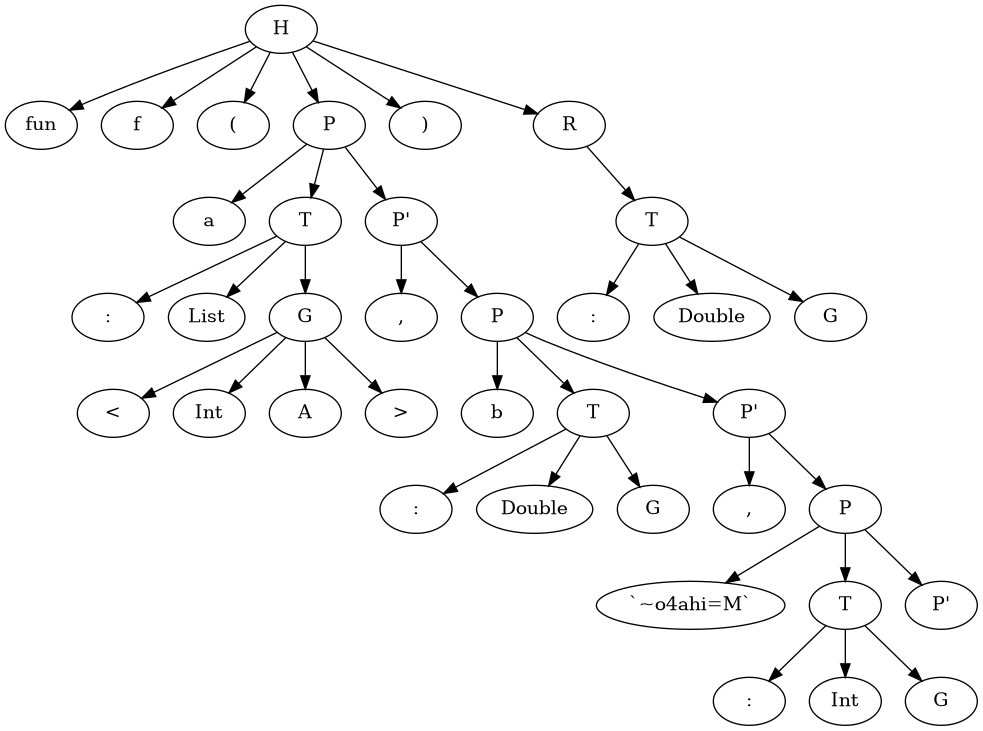
\includegraphics[scale=0.4]{lab2/tree.png}
    \caption{Пример дерева разбора для\\\texttt{fun f(a: Int, b: Double, `\~{}o4ahi=M`: Int):Double}}
\end{figure}

\inputminted[bgcolor=bg]{kotlin}{lab2/src/main/kotlin/Main.kt}

\section{Подготовка набора тестов}

\begin{center}
    \begin{tabular}{ll}\toprule
        Тест                                    & Описание                                     \\ \midrule
                                                & Пустой тест (должен произвести ошибку)       \\
        \texttt{fun f(a: Int, b: Bool): Double} & Небольшой случайный пример                   \\
        \texttt{fun f(a: Int, b: Bool)}         & Тест без возвращаемого типа                  \\
        \texttt{fun f(): Double}                & Тест без параметров                          \\
        \texttt{fun f()}                        & Тест без параметров и возвращаемого типа     \\
        \texttt{fuuun f()}                      & Тест с неверным ключевым словом \texttt{fun} \\
        \texttt{fun \_F1\_a2(`'g[4]VA?`: Int)}  & Тест с экранированным идентификатором        \\
        \texttt{fun f(a: Int):}                 & Тест с двоеточием для типа, но без типа      \\
        \texttt{fun f(a: Int): 1}               & Тест с неверным идентификатором              \\
        \texttt{fun f(a: 1)}                    & Тест с неверным идентификатором              \\
        \texttt{fun f(1: Int)}                  & Тест с неверным идентификатором              \\
        \texttt{fun 1()}                        & Тест с неверным идентификатором              \\
        \texttt{fun f(a: Int,)}                 & Тест с висящей запятой                       \\
        \texttt{fun f(, a: Int)}                & Тест с неверно расположенной запятой         \\
        \bottomrule
    \end{tabular}
\end{center}

\end{document}
